\chapter{XDG Development Kit}\label{ch:XDK}

\begin{figure}[!ht]
\begin{center}
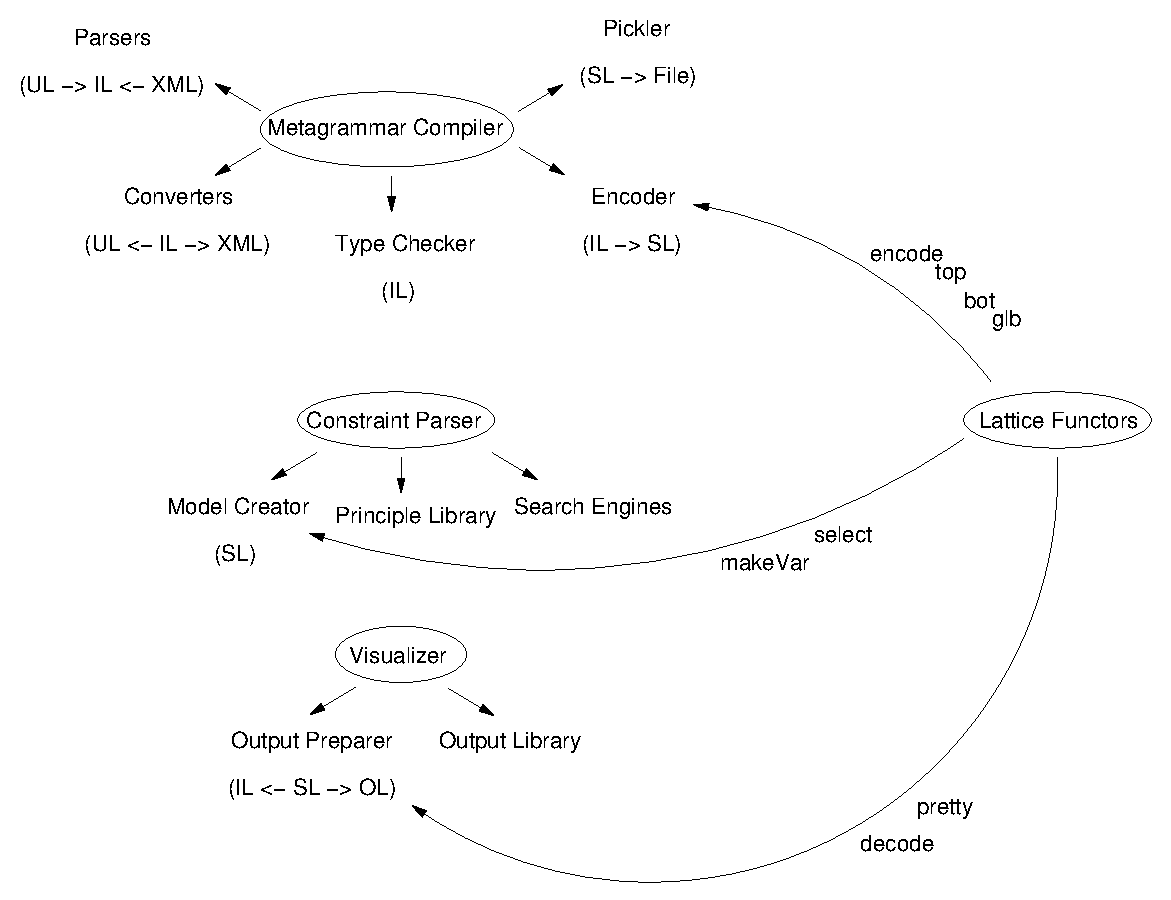
\includegraphics[width=11cm]{eps/xdk_architecture.eps}
\end{center}
\caption{Architektur von XDK}
\label{xdkarch}
\end{figure}

Das Extensible Grammar Development Kit (XDK) ist die Implementation
des XDG Grammatikformalismus. Mit Hilfe von XDK k\"onnen XDG
Grammatiken aufgeschrieben werden, und S\"atze mit der Grammatik
geparst werden bzw.\ es k\"onnen L\"osungen gefunden werden.

\section{Architektur}

Das XDK liefert verschiedene Werkzeuge um Grammatiken aufzuschreiben
und um L\"osungen f\"ur Eingabes\"atze zu finden. Darunter sind vor
allem die XDK Description Language, mit deren Hilfe Grammatiken
aufgeschrieben werden k\"onnen, und ein grafisches Interface um z.B.\
die L\"osungen anzuzeigen. Wie in Abbildung~\ref{xdkarch} zu sehen,
besteht XDK aus drei Hauptmodulen:
\begin{itemize}
\item dem Metagrammar Compiler, um die aufgeschriebene Grammatik f\"ur
  den Constraint Parser vorzubereiten
\item dem Constraint Parser, der die L\"osungen sucht
\item dem Visualisierer, der die Ergebnisse grafisch aufbereitet und
darstellt
\end{itemize}
Die Lattice-Funktoren stellen Funktionalit\"at f\"ur alle drei Module
bereit, u.a.\ Vererbung, die durch die \emph{greatest lower
bound}-Verbandsoperation modelliert wird (Metagrammar Compiler), das
Ausw\"ahlen von Lexikoneintr\"agen mithilfe des Selection Constraint
\cite{Duchier99}, \cite{Duchier03} (Constraint Parser), und die
Aufbereitung von L\"osungen (Visualisierer).

\subsection{Metagrammar Compiler}

Der Metagrammar Compiler transformiert Grammatiken, die mit Hilfe der
Description Language geschrieben wurden, in die Solver Language (SL),
mit der XDK intern arbeitet.  Bei der \"Ubersetzung in die Solver
Language werden unter anderem die Klassenhierarchien des Lexikons, die
XDG vorsieht und durch die Description Language aufgeschrieben werden
k\"onnen, aufgel\"ost, und f\"ur jedes Wort ein kompletter Eintrag
erstellt. Das Lexikon wird also flach gemacht. Die Description
Language stellt drei verschiedene Syntaxen zur Verf\"ugung:
\begin{enumerate}
\item Die User Language (UL), mit der XDG Grammatiken von Hand
  aufgeschrieben werden k\"onnen.
\item Die XML Language (XML) ist eine XML-basierte Sprache zur
  automatischen Generierung von Grammatiken.
\item Die Intermediate Language (IL) ist eine Sprache, die die
  Mozart/Oz Syntax verwendet, und die einerseits dazu gebraucht werden
  kann, Grammatiken automatisch zu generieren. Andererseits wird sie
  intern im XDK verwendet.
\end{enumerate}
Der Metagrammar Compiler kann auch Grammatiken aus IL in UL oder XML
umwandeln, sowie kompilierte SL Grammatiken in Dateien schreiben.  XML
und IL sind aufgrund ihrer Ausf\"uhrlichkeit nicht geeignet, um
Grammatiken von Hand zu schreiben.  Deshalb werden wir in den
folgenden Kapiteln nur noch die lesbare User Language betrachten.

Vor dieser Arbeit konnte in der XDK Description Language nur der
Multigraphtyp und das Lexikon beschrieben werden, nicht aber die
Prinzipien.  Die Prinzipien mussten bisher entweder aus der
vordefinierten Prinzipienbibliothek ausgew\"ahlt werden, \"ahnlich
einem Bausteinsystem, oder m\"uhsam von Hand selbst in Mozart/Oz
entwickelt werden:
$$
\begin{array}{r c c c l}
\text{Grammatik G = (} & \text{MT,} & \text{lex,} & \text{P} & \text{)} \\
 & \uparrow & \uparrow & \uparrow & \\
 & \text{\ding{52}} & \text{\ding{52}} & \text{\ding{55}} &
\end{array}
$$ Wie der Multigraphtyp und das Lexikon mit der XDK Description
Language aufgeschrieben werden, und wie die Prinzipien, die in der
Description Language fehlen, in XDK implementiert werden, werden wir
in den n\"achsten Kapiteln sehen.

\subsection{Constraint Parser}

\begin{figure}[!ht]
\begin{center}
\begin{tabular}{c c c c c}
\begin{tabular}{c} 
Grammatik in SL \\
Eingabesatz
\end{tabular}
& $\rightarrow$ & 
$\underbrace{
\begin{array}{c}
\text{Constraint}\\
\text{Satisfaction}\\ 
\text{Problem}
\end{array}
}_{
\begin{array}{c}
\text{Model Creator} \\
\text{und} \\
\text{Principle Library}
\end{array}}$ &
$\rightarrow$ & $\underbrace{\text{L\"osungen}}_{\begin{array}{c}\text{Search Engines}\end{array}}$

\end{tabular}
\end{center}
\caption{Constraint Parser}
\label{constraintparser}
\end{figure}

Der Constraint Parser baut aus der vom Metagrammar Compiler in die
Solver Language kompilierten Grammatik und einem Eingabesatz ein
Constraint Satisfaction Problem (CSP) mit Hilfe des Model Creator.
Dabei erweitert er das Constraint Satisfaction Problem um die
Prinzipien aus der vordefinierten Prinzipienbibliothek.  Die Search
Engines finden die L\"osungen des CSP. Dieser Ablauf ist in
Abbildung~\ref{constraintparser} illustriert.

\subsection{Visualisierer}

Der Visualisierer kann die vom Constraint Parser gefundenen L\"osungen
entweder grafisch darstellen, oder als {\LaTeX}-Quellcode. Wie die
Prinzipien ist auch der Visualisierer als Bibliothek implementiert. Es
lassen sich bequem neue Visualisierungsmodule hinzuf\"ugen.  Der
Visualisierer kann dabei kann nicht nur mit vollst\"andigen, sondern
auch mit partiellen L\"osungen umgehen.

\section{XDK Description Language}

Wir werden die XDK Description Language nicht komplett definieren,
sondern sie anhand eines Beispiels erkl\"aren. Ebenso werden wir im
Beispiel sehen, wie der Multigraphtyp und das Lexikon beschrieben
werden. Daf\"ur werden wir die CSD-Grammatik aus Kapitel~\ref{XDG}
verwenden, und zeigen, wie diese in XDK implementiert wird.

\subsection{Multigraphtyp-Definition}

\begin{figure}[!ht]
\begin{center}
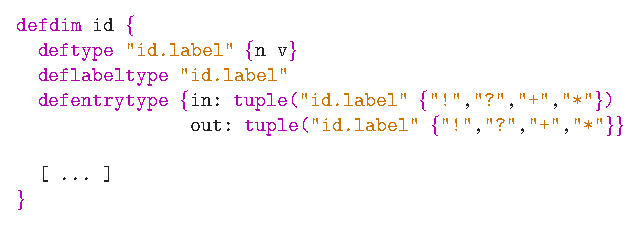
\includegraphics[scale=1.0]{eps/metatypbps}
\end{center}
%% \begin{center}
%% \begin{verbatim}
%% defdim id {
%%   deftype "id.label" {n v}
%%   deflabeltype "id.label"
%%   defentrytype {in: tuple("id.label" {!,?,+,*})
%%                 out: tuple("id.label" {!,?,+,*}}

%%   [ ... ]
%% }
%% \end{verbatim}
%% \end{center}
\caption{Multigraphtyp-Definition Beispiel: die Dimension ID der
CSD-Grammatik}
\label{metatypbps}
\end{figure}

Zuerst definieren wir den Multigraphtyp unserer Grammatik. In der XDK
Description Language k\"onnen hierzu Typen {\tt T} an Typnamen {\tt a}
gebunden werden mit dem Eintrag {\tt deftype a T}. Im Beispiel in
Abbildung~\ref{metatypbps} wird die Menge $\{n ~ v \}$ an den Typnamen
{\tt id.label} gebunden.  In der n\"achsten Zeile wird die Menge {\tt
id.label} als Menge der m\"oglichen Kantenbeschriftungen f\"ur die
ID-Dimension definiert ({\tt deflabeltype}).  Die beiden n\"achsten
Zeilen legen die lexikalischen Attribute der Knoten fest mit dem
Befehl {\tt defentrytype}. Das {\tt in}-Attribut hat z.B.\ als Typ
eine Menge aus Paaren, wobei jedes Paar zuerst einen Wert aus {\tt
id.label} hat, gefolgt von einem Atom aus der Menge $\{ \dq ! \dq ~
\dq ? \dq ~ \dq + \dq ~ \dq * \dq \}$.

\subsection{Lexikon-Definition}

F\"ur die Beschreibung des Lexikons k\"onnen lexikalische Klassen
verwendet werden, die eine Repr\"asentation von lexikalischen
Eintr\"agen sind, die \"uber beliebig viele Variablen abstrahieren
k\"onnen. Sie sind damit \"ahnlich zu Templates in anderen
Grammatikformalismen wie PATR-II \cite{Shieber84}. Au{\ss}erdem kann
mit den lexikalischen Klassen eine Vererbungshierarchie aufgebaut
werden. Als Beispiel entwickeln wir ein Lexikon f\"ur die
CSD-Grammatik. Wir definieren zwei lexikalische Klassen: eine f\"ur
Verben und eine f\"ur Nomen (vgl.\ Abbildung~\ref{csdlexicon}).

Die Klasse f\"ur Verben sieht wie folgt aus. Sie abstrahiert \"uber
die Variable {\tt Word}, die das Wort des lexikalischen Eintrags
repr\"asentiert. W\"orter werden den Lexikoneintr\"agen \"uber das
Attribut {\tt word} auf der XDK-eigenen {\tt lex}-Dimension
zugeordnet:
\begin{center}
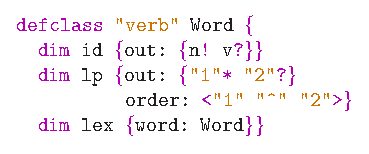
\includegraphics[scale=1.0]{eps/verb}
\end{center}
%% \begin{verbatim}
%% defclass "verb" Word {
%%   dim id {out: {n! v?}}
%%   dim lp {out: {"1"* "2"?}
%%           order: <"1" "^" "2">}
%%   dim lex {word: Word}}
%% \end{verbatim}

Die Klasse f\"ur die Nomen sieht so aus:
\begin{center}
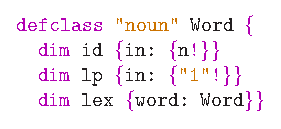
\includegraphics[scale=1.0]{eps/noun}
\end{center}
%% \begin{verbatim}
%% defclass "noun" Word {
%%   dim id {in: {n!}}
%%   dim lp {in: {"1"!}}
%%   dim lex {word: Word}}
%% \end{verbatim}

Im folgenden Schritt benutzen wir die lexikalischen Klassen. Wir
definieren mit dem Schl\"usselwort {\tt defentry} zuerst einen Eintrag
f\"ur Verben, die als Wurzelknoten vorkommen:
\begin{center}
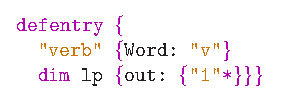
\includegraphics[scale=1.0]{eps/verbroot}
\end{center}
%% \begin{verbatim}
%% defentry {
%%   "verb" {Word: "v"}
%%   dim lp {out: {"1"*}}}
%% \end{verbatim}
Der Eintrag erbt von der lexikalischen Klasse {\tt verb}, \"ubernimmt
damit alle Attribute der Klasse {\tt verb}, und erlaubt zus\"atzlich
auf der Dimension {\tt lp} noch beliebig viele ausgehende Kanten mit
dem Label {\tt 1}.

Ein Verb, das kein Wurzelknoten ist, w\"urde die Klasse {\tt verb}
noch um zwei eingehende Kante erg\"anzen, so dass das Verb auf beiden
Dimensionen genau ein Dependent eines Verbes ist:
\begin{center}
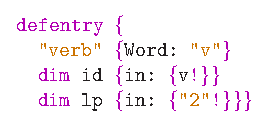
\includegraphics[scale=1.0]{eps/verbdependent}
\end{center}
%% \begin{verbatim}
%% defentry {
%%   "verb" {Word: "v"}
%%   dim id {in: {v!}}
%%   dim lp {in: {"2"!}}}
%% \end{verbatim} 

Ein konkretes Nomen muss die Klasse {\tt noun} gar nicht erweitern,
sondern nur davon erben, dementsprechend kurz ist der Eintrag f\"ur
das Nomen n:
\begin{center}
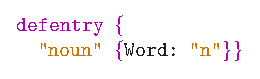
\includegraphics[scale=1.0]{eps/nounentry}
\end{center}
%\begin{verbatim}
%defentry {
%  "noun" {Word: "n"}}
%\end{verbatim}

Der Metagrammar Compiler erzeugt aus der Klassenhierarchie und den
Eintragsdefinitionen Lexikoneintr\"age, so, als h\"atten wir das
Lexikon nicht mit Hilfe von Klassen implementiert, sondern f\"ur jedes
Wort alle Attribute angegeben. Er macht das Lexikon also flach:
\begin{center}
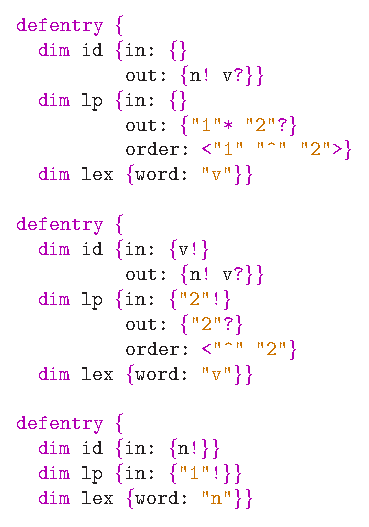
\includegraphics[scale=1.0]{eps/lexflat}
\end{center}
%% \begin{verbatim}
%% defentry {
%%   dim id {in: {}
%%           out: {n! v?}}
%%   dim lp {in: {}
%%           out: {"1"* "2"?}
%%           order: <"1" "^" "2">}
%%   dim lex {word: "v"}}

%% defentry {
%%   dim id {in: {v!}
%%           out: {n! v?}}
%%   dim lp {in: {"2"!}
%%           out: {"2"?}
%%           order: <"^" "2"}
%%   dim lex {word: "v"}}

%% defentry {
%%   dim id {in: {n!}}
%%   dim lp {in: {"1"!}}
%%   dim lex {word: "n"}}
%% \end{verbatim}

\subsection{Prinzipien-Instanziierung}~\\

\begin{figure}[!ht]
\begin{center}
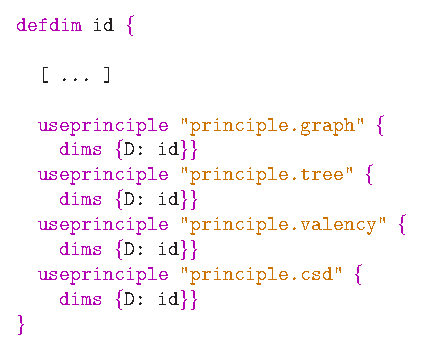
\includegraphics[scale=1.0]{eps/useprinciples}
\end{center}
%% \begin{center}
%% \begin{verbatim}
%% defdim id {

%%   [ ... ]  

%%   useprinciple "principle.graph" {
%%     dims {D: id}}
%%   useprinciple "principle.tree" {
%%     dims {D: id}}
%%   useprinciple "principle.valency" {
%%     dims {D: id}}
%%   useprinciple "principle.csd" {
%%     dims {D: id}}
%% }
%% \end{verbatim}
%% \end{center}
\caption{Prinzipien-Instanziierung Beispiel: Die Dimension ID der CSD-Grammatik}
\label{definstant}
\end{figure}

Bei der Prinzipien-Instanziierung wird eine Teilmenge der Prinzipien
der Prinzipienbibliothek ausgew\"ahlt, um die
Wohlgeformtheitsbedingungen der Grammatik festzulegen. Um
wiederverwendbar zu sein, abstrahieren viele der Prinzipien aus der
Prinzipienbibliothek \"uber die Dimensionen, die sie
einschr\"anken. Diese \emph{Dimensionsvariablen} werden bei der
Instanziierung an konkrete Dimensionen gebunden.  In
Abbildung~\ref{definstant} werden so mit dem Schl\"usselwort {\tt
useprinciple} die Prinzipien {\tt principle.graph}, {\tt
principle.tree}, {\tt principle.valency} und {\tt principle.csd}
instanziiert, und jeweils die Dimensionsvariable {\tt D} an die
konkrete Dimension {\tt id} gebunden.

\section{Constraint Parser}

Das Herzst\"uck vom XDK, der Constraint Parser, muss zum Finden von
L\"osungen Multigraphen modellieren und die Prinzipienbibliothek
implementieren. Wie das funktioniert, wird in den n\"achsten Kapiteln
gezeigt.

\subsection{Modellierung von Multigraphen}

\begin{figure}[!ht]
\begin{center}
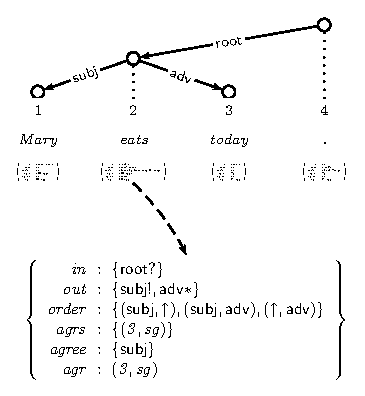
\includegraphics[scale=1.0]{eps/syn1mag_xdag}
\end{center}
\caption{Dependenzgraph f\"ur Peter eats today}
\label{depbsp}
\end{figure}

Der Constraint Parser modelliert Multigraphen mithilfe von endlichen
Mengen von nat\"urlichen Zahlen. Der Dependenzgraph aus Abbildung
\ref{depbsp} z.B.\ hat vier Knoten. Der Knoten f\"ur das Wort eats hat
zwei T\"ochter. Bei der Modellierung des Dependenzgraphen wird f\"ur
jeden Knoten ein \emph{Knotenrecord} erzeugt, der die ausgehenden
Kanten als T\"ochtermenge repr\"asentiert. F\"ur das Wort eats sieht
der Knotenrecord so aus:

\Equsl{c}{1.0}{%
  \begin{rec}
    \Findex&=&2\\
    \Fword&=&\Str{eats}\\
    \FnodeSet&=&\Set{1,2,3,4}\\
    \Fmodel&=&
    \begin{rec}
      \FdaughtersL&=&
      \begin{rec}
        \La{adv}&=&\Set{3}\\
        \La{root}&=&\Set{}\\
        \La{subj}&=&\Set{1}
      \end{rec}
    \end{rec}
  \end{rec}}{solver:eq:eats}

Das Attribut index bezeichnet den Index des Knotens, der den Knoten
eindeutig benennt. Das Attribut nodeSet enth\"alt alle Knoten,
bzw.\ deren Indizes, die der Dependenzgraph enth\"alt. Der Unterrecord
daughtersL enth\"alt f\"ur jedes Kantenlabel die Knoten, die \"uber
dieses Label direkt \"uber eine Kante erreicht werden k\"onnen.

In Mozart/Oz Syntax wird der Record so dargestellt:
\Einc{eps/eats1_oz}{1.0}{solver:eq:eats1}
Da in Mozart/Oz jeder Record
einen Namen haben muss, werden die {\tt o} Zeichen als Dummynamen
verwendet. Mengen werden in geschweiften Klammern geschrieben, gefolgt
von Ihrer Kardinalit\"at.

Der Constraint Parser erzeugt f\"ur jeden Knoten noch weitere Mengen
neben daughtersL. Diese sind in Anhang, Abschnitt~\ref{cpmengen}
aufgelistet. Die Mengen werden vor allem f\"ur die bequemere und
effizientere Implementation der Prinzipien verwendet.  Der komplette
Record des Knotens f\"ur das Wort eats mit allen Mengen sieht dann so
aus:

\Einc{eps/eats2_oz}{1.0}{solver:eq:eats2}

Die Attribute werden in den Unterrecords attrs (nichtlexikalische Attribute) und entry (lexikalische Attribute) modelliert. Der Knoten f\"ur das Wort eats mit den Attributen sieht dann so aus:

\Einc{eps/eats4_oz}{1.0}{solver:eq:eats4}

Um einen kompletten Multigraph zu modellieren bekommt der Record f\"ur
jede Dimension ein Attribut mit dem Namen der Dimension. Dieses
Attribut hat als Wert den {\tt model}-Unterrecord des Dependenzgraphen
der Dimension.

\subsection{Modellierung von Prinzipien}

Ein Prinzip besteht aus zwei Teilen, der Prinzipiendefinition und
einer Menge von Node-Constraint-Funktoren. 

Bei der Prinzipiendefinition wird der Name des Prinzips definiert,
eine Menge von Dimensionsvariablen, \"uber die das Prinzip
abstrahiert, und eine Menge von Node-Constraint-Funktoren und deren
Priorit{\"a}t, die das Prinzip implementieren. Z.B.\ sieht die
Prinzipiendefinition des CSD-Prinzipes so aus:
%\Einc{eps/defValency_ul}{1.0}{solver:eq:defValency}
\begin{center}
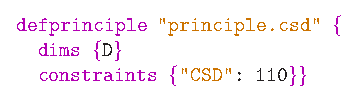
\includegraphics[scale=1.0]{eps/defprinciple}
\end{center}
%% \begin{verbatim}
%% defprinciple "principle.csd" {
%%   dims {D}
%%   constraints {"CSD": 110}
%% \end{verbatim}
Der Name des Prinzipes ist ``principle.csd''. Es abstrahiert \"uber
die Dimensionsvariable D und benutzt den Node-Constraint-Funktor CSD
mit Priorit\"at 110. Die Priorit\"aten legen die zeitliche Reihenfolge
der Constraint-Anwendung fest---je h\"oher die Priorit\"at, desto eher
wird der Constraint angewandt. Damit lassen sich in manchen F\"allen
Effizienzgewinne erzielen.

Die Node-Constraint-Funktoren werden direkt als Oz-Prozeduren
implementiert, die den Namen {\tt Constraint} tragen. Sie haben keinen
R\"uckgabewert. Jeder Funktor hat vier Argumente:
\begin{enumerate}
\item Nodes: Die Liste der Knotenrecords, die den Multigraphen
repr\"asentieren
\item G: Die Grammatik
\item GetDim: Eine Funktion, die Dimensionsvariablen konkrete Dimensionen
zuweist
\end{enumerate}

%\Finc{eps/In1_ozn}{1.0}{$\Ulo{{\Dq}In{\Dq}}$ node constraint
%  functor}{solver:fig:In1}
 
\subsubsection{Beispiel: CSD-Prinzip}

\begin{figure}
\begin{center}
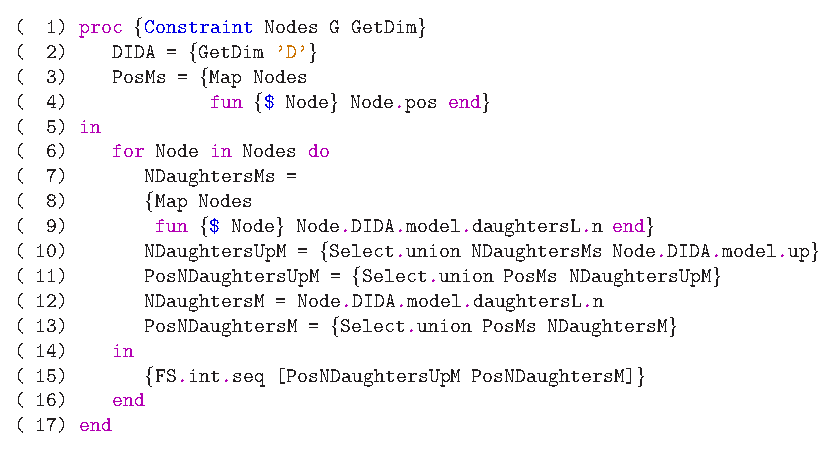
\includegraphics[scale=1.0]{eps/csdconstraint_n}
\end{center}
%% \begin{verbatim}
%% proc {Constraint Nodes G GetDim}
%%   DIDA = {GetDim 'D'}
%%   PosMs = {Map Nodes 
%%            fun {$ Node} Node.pos end}
%% in
%%   for Node in Nodes do
%%     NDaughtersMs = 
%%       {Map Nodes
%%          fun {$ Node} Node.DIDA.model.daughtersL.n end}
%%       NDaughtersUpM = {Select.union NdaughtersMs Node.DIDA.model.up}
%%       PosNDaughtersUpM = {Select.union PosMs NDaughtersUpM}
%%       NDaugtersM = Node.DIDA.model.daughtersL.n
%%       PosNDaugtersM = {Select.union PosMs NDaughtersM}
%%   in
%%     {FS.int.seq [PosNDaughtersUpM PosNDaughtersM]}
%%   end
%% end
%% \end{verbatim}
\caption{``CSD'' Node-Constraint-Funktor}
\label{CSDFunctor}
\end{figure}

In Abbildung~\ref{CSDFunctor} ist als Beispiel der
Node-Constraint-Funktor ``CSD'' des CSD-Prinzips zu sehen. In Zeile 2
holt sich der Funktor die konkrete Dimension, die durch die
Dimensionsvariable {\tt D} repr\"asentiert wird. In der dritten und
vierten Zeile wird eine Liste mit den Positionsmengen der Knoten
erstellt.

In der {\tt for}-Schleife \"uber die Knoten werden in jedem Durchgang
die n-Dependenten aller Knoten bestimmt (Zeile 7--9). In Zeile 10
werden die n-Dependenten der Vorg\"anger des aktuellen Knotens {\tt
Node} bestimmt, und in Zeile 11 deren Positionen ermittelt.  In Zeile
12 werden die n-Dependenten des aktuellen Knotens bestimmt, und in
Zeile 13 deren Position. In Zeile 15 schlie{\ss}lich wird mit Hilfe
der Funktion {\tt FS.int.seq} ausgedr\"uckt, dass die Positionen der
n-Dependenten der Vorg\"anger des aktuellen Knotens immer vor den
Positionen der n-Dependenten des aktuellen Knotens stehen m\"ussen.
Die Funktion {\tt FS.int.seq} bekommt zwei disjunkte Mengen aus den
nat\"urlichen Zahlen, und pr\"uft, ob alle Elemente der ersten Menge
kleiner sind als die Elementen der zweiten Menge.

In dem Beispiel ist gut zu sehen, wie die verschiedenen Mengen aus den
Modellen verwendet werden. Allerdings sieht man anhand dieses
Beispiels auch, dass die Implementierung eines Prinzips nicht trivial
ist und u.U.\ kaum mehr \"Ahnlichkeiten mit dessen Formalisierung hat
(Vgl.:~\ref{treeprinciple}). Damit kommen wir zur Problemstellung.

\section{Problemstellung}

Wir haben gesehen, wie der Multigraphtyp und das Lexikon und einer XDG
Grammatik mit Hilfe der XDK Description Language aufgeschrieben werden
k\"onnen. Leider kann der letzte Teil einer XDG-Grammatik, die
Prinzipien, nicht so sch\"on entwickelt werden.  Die XDK Description
Language erlaubt nur, Prinzipien aus einer Prinzipienbibliothek
auszuw\"ahlen, nicht aber neue zu entwickeln.  Um neue Prinzipien
hinzuf\"ugen zu k\"onnen, muss der Grammatikschreiber sehr vertraut
sein mit Mozart/Oz-Constraintprogrammierung, was man bei typischen
Grammatikschreibern wie z.B.\ Linguisten nicht voraussetzen kann.

Hier besteht also eine gro{\ss}e L\"ucke zwichen der Formalisierung
(XDG) und der Implementierung (XDK) des Grammatikformalismus. Diese
L\"ucke wird in den n\"achsten Kapiteln geschlossen, wo die
Entwicklung eines Werkzeugs namens PrincipleWriter (PW) beschrieben
wird. Der PW erlaubt es, Prinzipien als Formeln in First-Order Logik
aufzuschreiben, und diese dann automatisch in Mozart/Oz Constraints
umzusetzen.
